
\documentclass{sig-alternate}
  \pdfpagewidth=8.5truein
  \pdfpageheight=11truein

\usepackage{cite}
\usepackage{listings}
\usepackage{booktabs}
\usepackage{color}
\usepackage{balance} % Add this back in. Probably needed during camera ready.
\usepackage{url}
\usepackage{times} % Used for formatting formatting url footnotes
\urlstyle{same} % Used for formatting formatting url footnotes

%\usepackage{array}
%\usepackage{subfigure}
%\usepackage{hyperref}
%\usepackage{tikz}
%\usepackage{pgfplots}0


%%% Used to anonymoyze paper
\newif\ifisnopii
%\isnopiitrue % change to true/false to remove personally identifiable information (pii)
\isnopiifalse



\setlength{\abovecaptionskip}{6pt plus 3pt minus 2pt} % Space over captions
%\setlength{\belowcaptionskip}{6pt plus 3pt minus 2pt} % Space under captions

\newcommand{\todo}[1]{\textcolor{cyan}{\textbf{[#1]}}}
\newcommand{\sam}[1]{\textcolor{red}{{\it [Sam says: #1]}}}
\newcommand{\dan}[1]{\textcolor{blue}{{\it [Dan says: #1]}}}


\begin{document}
%
% --- Author Metadata here ---
\conferenceinfo{SAC'15}{April 13-17, 2015, Salamanca, Spain.}
\CopyrightYear{2015} % Allows default copyright year (2002) to be over-ridden - IF NEED BE.
\crdata{X-XXXXX-XX-X/XX/XX}  % Allows default copyright data (X-XXXXX-XX-X/XX/XX) to be over-ridden.
% --- End of Author Metadata ---

\title{A Project Component in a Web Engineering Course}
\ifisnopii % turn on/off pii
\author{
%
% 1st. author
\alignauthor
Daniel~E.~Krutz~and~Samuel~A.~Malachowsky\\ 	
	\affaddr{Software Engineering Department}\\
       \affaddr{Rochester Institute of Technology}\\
       \affaddr{1 Lomb Memorial Drive}\\
       \affaddr{Rochester, NY, USA} \\
       \email{\{dxkvse, samvse\}@rit.edu}
} % Must not be a space above this

\else % turn on/off pii
\author{
%
% 1st. author
\alignauthor
xxxxxxxxxxxxxxx\\ 	
	\affaddr{xxxxxxxxx}\\
       \affaddr{xxxxxxxxx}\\
       \affaddr{xxxxxxxxx}\\
       \affaddr{xxxxxxxxx, xx, xxx} \\
       \email{xxxxxx@xxxxx.xxx}
       \alignauthor
xxxxxxxxxxxxxxx\\
        \affaddr{xxxxxxxxx}\\
       \affaddr{xxxxxxxxx}\\
        \affaddr{xxxxxxxxx}\\
       \affaddr{xxxxxxxxx, xx, xxx} \\
       \email{xxxxxx@xxxxx.xxx}
} % Must not be a space above this
\fi % end turn on/off pii

\maketitle
\begin{abstract}
\todo{latest version in Google Docs}
Web applications are an extremely important and ubiquitous part of today's world. Students must not only know how to develop them from a technical perspective, but in doing so need to understand how to follow the proper principles of software engineering - delivering the project on time, on budget, and in a high quality manner.

At the Department of Software Engineering at \ifisnopii the Rochester Institute of Technology\else xxxxxx xxxxxx xxxxxx\fi, we currently offer a Web Engineering course which includes a significant project component requiring students to use a variety of contemporary technologies and resources to create a robust web application. It includes multiple releases and requires the use of proper web engineering principles.

This innovative project component has received significant praise from both students and faculty members while fulfilling an emerging area of our curriculum. Students enjoy the real-world nature of the project and the ability to work with contemporary technologies in a format which closely mimics what they will see in industry. This paper outlines the educational objectives, project details, and some sample project results of our class offering. The goal of this work is to share the project, its importance, and lessons learned for use at other institutions with similar educational goals.

\end{abstract}




\category{K.3.2}{Computers and Education}Computers and Information
Science Education- Computer science education; Curriculum

%\terms{Design, Human Factors}

\keywords{Web Engineering, Software Engineering Education, Software Project}

\begin{table*}[t]
  \centering
  \caption{Weekly Topics \& Project Deliverables}
     \begin{tabular}{ c | l | l | l}
 \bfseries Week & \bfseries Classroom Topics & \bfseries Project Deliverables & \bfseries Project Point Total  \\ \hline \hline
	\bfseries 1 & Course Introduction, Introduction to Web Engineering & Team Formation & 0\%\\ \hline
	\bfseries 2 & Introduction to Web Development Technologies & \\ \hline
	\bfseries 3 & Javascript, JQuery & Requirements Documents & 10\\ \hline
	\bfseries 4 & Web Services & \\ \hline
	\bfseries 5 & Web Testing & Design Documents, Test Plan & 10\\ \hline
	\bfseries 6 & Exam, Twitter Bootstrap & Beta Release & 3\\ \hline
	\bfseries 7 & R1 Presentations & Release 1 (R1) & 20\\ \hline
	\bfseries 8 & Introduction to Databases & R1 Post Mortem & 4\\ \hline
	\bfseries 9 & HTML5 & \\ \hline
	\bfseries 10 & Security - Abuse \& Misuse,  Threat Modeling& \\ \hline
	\bfseries 11 & R2 Presentations,  Security - Defensive Coding, SQL Injection & R2 & 20\\ \hline
	\bfseries 12 & Exam, Usability in Web Applications & R2 Post Mortem & 4\\ \hline
	\bfseries 13 & Analysis of Web Traffic & \\ \hline
	\bfseries 14 & Emerging Web Technologies & \\ \hline
	\bfseries 15 & R3 Presentations, Final Exam & Presentation, R3, R3 Post Mortem & 5, 20, 4\\
  \end{tabular}
  \label{table:weeklytopics}

\end{table*}

\section{Introduction}

Creating high quality web applications on time and on budget can be in many ways more difficult than traditional application development. Developers must not only master web development technologies, but different methodologies as well. Web-deployed development is likely to have a significantly higher amount of all three types of maintenance (corrective, adaptive, and perfective) by its very nature; evolvability and ease of deployment are a major reason why it is so popular. In addition to focusing on maintainability, developers need to balance the concepts of uptime, security, worldwide availability, and accessibility with a torrent of different browsers, devices, and screen resolutions currently in use and in the development pipeline.

Web engineering is defined as the systematic, disciplined, and quantifiable approach to development, operation, and maintenance of web-based systems and applications ~\cite{Schummer:2005:TDS:1149293.1149369,Mendes:2003:ACF:858403.858417,Reif:2005:WWE:1060745.1060849}. While similar to software engineering, the concept of web engineering differs in several key areas~\cite{Ginige:2002:WEM:568760.568885}. A higher emphasis is placed on growth and change, compressed schedules, performance criticality, and small teams working on very short schedules~\cite{Deshpande:2002:WE:2011098.2011101}. While many institutions offer classes directed towards developing web applications or software engineering, very few offer courses in web engineering - the successful combination of the two concepts ~\cite{tufts_webengineering,csun_webengineering}. Because of the critical elements described above, the application of engineering principles to this particular type of development is critical.

At the Department of Software Engineering at \ifisnopii the Rochester Institute of Technology (RIT)\else xxxxxx\fi, we offer a Web Engineering course to help meet the demands that students would face when tasked with creating web applications. The purpose of this course is to instruct students in using proper web engineering principles and to allow them to practice doing so with a prominent course project. This project component includes teams of 3-5 students, runs the entire (15 week) semester, and involves creating a web application in multiple iterations using a variety of contemporary technologies and resources.

The goals of the project are to reinforce course concepts, allow students to gain experience creating web applications, and the application of web engineering concepts. Secondary goals include reinforcement of in a team skills and the opportunity to use current technologies. Student teams are expected to fulfill all steps of the software development lifecycle including the successful creation of all necessary requirement, design, test, and deployment artifacts, and development of the product using proper web engineering principles. This project has proven to be invaluable at reinforcing academic concepts discussed in the classroom as well as providing an enjoyable real-world experience for the students.

The rest of the paper is organized as follows: Section~\ref{sec: aboutcourse} describes the course including learning objectives. Section~\ref{sec: aboutproject} provides an overview of the project detailing requirements, deliverables and evaluation methods. Section~\ref{sec: studentfeedback} relates a sample project and some student feedback, Section~\ref{sec: relatedwork} presents some related works. Section~\ref{sec: futurework} describes challenges and future work, and Section~\ref{sec: summary} concludes the paper with a summary.

\section{About the course}
\label{sec: aboutcourse}

%
% Why there was a need for the course
% Web Engineering is different than software engineering
% Describe the background of the students
% Discuss Weekly topics
%	Introduce a few potential new weekly topics as well


The Web Engineering course has been offered at \ifisnopii RIT \else xxxxxx \fi for three years, with the primary goal being to instruct students in how to properly apply software engineering principles to the creation of web applications. While this is an engineering and not a programming course, specific technologies such as .NET\footnote{http://microsoft.com/net} and jQuery\footnote{http://jquery.com/} are discussed and and concepts such as web services and security are covered. Students are primarily evaluated on their comprehension of engineering principles and not specific technologies or programming abilities.

The students taking the course are typically upper-level Software Engineering students and have a reasonably high level of development experience. A good portion of the students are very experienced with web development - having gained expertise either through personal projects or internships. Typically one third have extensive experience, one third have some experience, and the remaining third have little or no exposure. Exams and homework are two thirds of the final grade, and the project is one third. Prerequisites include Introduction to Software Engineering, Personal Software Engineering, and some basic programming courses.

Some of the biggest ares of emphasis include customer elicitation skills, requirements documentation, and acceptance testing within the context of web engineering.  The weekly topics, project deliverables, and suggested project point totals of the course are shown in Table~\ref{table:weeklytopics}; further details may be found on the course website\footnote{\ifisnopii\url{http://www.se.rit.edu/~swen-344/}\else http://xxxxxx \fi}. Instructors are encouraged to deviate from our course plan as they see fit and as new technologies and concepts become prominent.


\begin{figure*}[ht!]
\centering
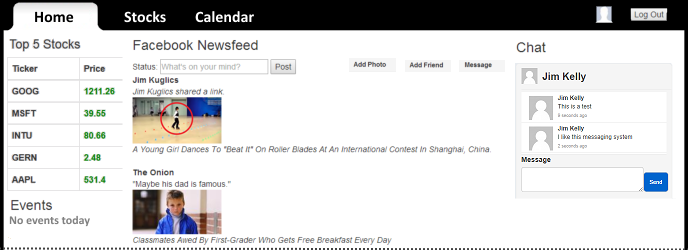
\includegraphics[width=1.0\textwidth]{images/R2b.png}
\caption{A Sample Completed Student Project}
\label{fig:website1}
\end{figure*}

\section{About the project}
\label{sec: aboutproject}

A group project is an important aspect of the course; research has found projects to be extremely beneficial to student learning~\cite{Schummer:2005:TDS:1149293.1149369,Guo:2009:GPS:1516546.1516579,Coppit:2005:LTP:1047124.1047400}. The project lasts the entire term of the course (15 weeks), and has student teams creating deliverables throughout. Team size is targeted to 3-5 students, as this is often the size of groups in industry and has been found to be conducive to student learning in previous research~\cite{Guo:2009:GPS:1516546.1516579,Petkovic:2006:TPS:1140124.1140202}. For simplicity and student support purposes, a web technology platform should be chosen by the instructor. For the last three years, we have chosen the Microsoft .NET framework as the core of the project, although we expect other institutions to select the technology based upon preference and student competency.

The main premise of the project is for each group to create a web portal using both custom-built and already existing components.  This is accomplished through web service and Application Programming Interface (API) calls, with possible sources including Google's, FaceBook's, and Yahoo's APIs.

\subsection{Project Requirements}

When crafting the course project, several considerations were at hand. First, we wanted it to represent a real-world product, using-real world technologies. This is important since the goal of the project is to emulate what the students would see in their careers after college. Additionally realistic development goals help to further challenge and encourage students~\cite{Schummer:2005:TDS:1149293.1149369,Marmorstein:2011:OSC:1999747.1999823,Tadayon:2004:SEB:1050231.1050248,VanderDuim:2007:GPE:1248820.1248900,Hayes:2002:ESE:872751.873465}. Second we wanted to foster student interest in the project. Developing a solution using APIs from well-known and respected companies proved exciting to the students. This enthusiasm has helped them to remain focused and drive their desire to learn and apply ingenuity.

The instructor takes on two distinct roles for the project: teacher and customer. The way the customer reacts to student questions significantly differs depending on what role the instructor is currently playing. While representing the role of teacher, the instructor gives project advice and answers technical questions whenever possible. As the customer, an attempt is made to mimic a client in the real world, and students are encouraged to clarify requirements as such. So that students may understand which role the instructor is playing, they are encouraged to ask whenever they are unsure and begin their statements with ``As the customer'' or ``As the teacher.''

The goal of the project is to create a personalized web portal that would be customized for each user. We choose to require that the user be able login with their Facebook account, as Students of the millennial generation have been found to be more engaged with programming projects that have social relevance~\cite{Meneely:2008:RRE:1384271.1384276}. Once the user has logged into the application, they are to be exposed to several pieces of personal, customizable information. Perhaps the most significant is an area on the main page which is very similar to the wall in the traditional Facebook application. For this section, students are asked to again tie into the Facebook API to retrieve the necessary data. They are required to modify the appearance of these items and apply aspects of usability covered in the course. Various other Facebook APIs such as photo albums, chatting with friends, and status updates were used in similar ways.


In addition to the relatively simple API interaction, the students are also required to write custom software that has its own functionality and also interacts with external data services or feeds. One example is a simple stock/share price module requiring the user to enter a stock that they have fictitiously purchased along with the purchase price and number of shares. This information is to be stored in a student created MS-SQL database and information such as the current share price is to be retrieved from a third party web service. The student's page is expected to display the current stock price, the day's high and low price, and the amount of money the investment has made or lost for the user so far. A chart is also to be displayed for the stock, retrieved using an external feed of the group's choice. Other potential aspects of the application include a weather-based component and a chat feature.  The development cycle has a secondary goal of familiarizing students with HTML5, javascript, database design, and the use of libraries such as Twitter Bootstrap~\footnote{http://getbootstrap.com/} and jQuery. A sample end-result screenshot is shown in Figure~\ref{fig:website1}.

Teams are also expected to write their code in a clean manner while using a version control system of their choice, such as Git~\footnote{http://git-scm.com/}. Since teams are to produce multiple releases, each team is provided with a Windows Server virtual machine to deploy their project to, and are expected to produce and adhere to a robust deployment strategy. Finally, teams are required to use proper defensive coding practices to protect against SQL injection and cross-site scripting attacks. Instructors may choose to place more emphasis on specific aspects such as usability, security, testing, etc.


\subsection{Weekly Actions \& Deliverables}
In order to mimic the iterative nature of typical web application development cycles, we require teams to submit multiple project releases. These submissions also serve to reinforce the importance of maintainability and extensibility in web applications. While we encourage instructors to deviate from this plan as they see fit, we have outlined our deliverables and project releases below, based on a 15 week semester.  Suggested timing and point totals are listed in Table~\ref{table:weeklytopics}.\\ \\


\textbf{Week 1: Team Formation}\\
Teams are formed using an on-line survey where students are encouraged to indicate who they would and would not like to work with and their level of level of experience with web development and software engineering.  The instructor's goal is to to create balanced teams who are likely to work well together.

Each team is required to self-assign several roles including team coordinator, development coordinator, and testing coordinator. In our case, the course is comprised of upper level students making self-appointed roles appropriate; in the case of more novice students, the instructor may want to appoint team roles, possibly choosing to rotate them in order to allow each student to experience each role.
 \\

\textbf{Week 3: Requirements Documents}\\
Students are provided with a requirements document template which they modify based on their conversations with the customer/instructor. As with all project artifacts, teams are expected to keep these documents up to date for with each release throughout the term.

The grading on these initial document deliverables is not aimed at ensuring that the teams have a completely accurate document on their first attempt. The main goal is to have followed the proper guidelines for producing these deliverables and producing an adequate effort in creating them as accurately as possible. During the second half of the class, each team is given the opportunity to meet with the instructor to elicit requirements and to ask general project questions. In this and future interactions, the students are also able to negotiate expectations with the customer. They are encouraged to show prototypes, screenshots, and anything else they deem useful to the customer. The goal is not to limit customer interaction or punish inquisitions as long as they are reasonable, rather the aim is to encourage customer interaction and elicitation.\\

\textbf{Week 5: Design Documents \& Test Plan}\\
As with the requirements document, teams are provided a template design document and are expected to use the requirements they've been provided and elicited from the customer as input in its enhancement. Some expected document components include UML diagrams (state, sequence, and class), interface design, and basic database design. Teams are also expected to create a test plan for their project. In our course offerings, teams are instructed to create acceptance tests in a simple excel document. Instructors may choose to have teams use a more robust tool should they see fit. \\

\textbf{Week 6: Beta Release}\\
The initial project release is intended to be a lightly scrutinized preview of Release 1 (R1). If time allows, Instructors are encouraged to allow teams to conduct a short 5 minute demo of their applications and a basic progress report, eliciting feedback from their classmates. In our case, students have enjoyed seeing the progress of their classmates and gaining this extra feedback before their first major release.\\

\textbf{Week 7: Release 1 (R1)}\\
At this time, teams are asked to deliver a partially working version of their application and a 15 minute presentation. Teams are also expected to submit all updated project artifacts including the requirements document, design document, and test plan. Some key deliverables are basic connections with the external APIs, a deployment strategy, and cursory implementation. We do not evaluate usability or database setup for this initial release.

The Software Engineering Department at \ifisnopii RIT \else xxxxxx \fi places a large emphasis on the student skills of public speaking, presentation, and internal and external communication. With the first release, each group is asked to give a 15 minute presentation highlighting some of the major aspects of their product and some of the technologies they have encountered. Other aspects of discussion are team roles and dynamics, a short demonstration of their application, and plans for the second release. The presentation is oriented as a progress report for the customer.

We ask teams to identify any missing features or requirements not able to be delivered for the initial release. In order to help persuade the students to divulge these undelivered items, they are told they will be penalized much less significantly for any items that they have declared to have missed (as opposed to the instructor/customer finding them). This forces the students to take ownership of their mistakes and be open and honest with their customers, which we feel is an especially important concept once the students graduate to the real world. Hopefully these self-identified problem areas are addressed by the team and defeated in upcoming releases. Assisting in this, students are also required to complete an online, 360$^{\circ}$ survey rating their teammates and themselves in order to identify problematic areas and team members who are not contributing as much as they should to the project.

Teams may be evaluated upon the quality of their presentation, updated documentation, and created software.  Scores may be influenced by team contribution, adherence to process (i.e. using the repository effectively), and metrics such as defect density.\\

\textbf{Week 8: R1 Postmortem}\\
Each team creates a self-reflection document containing that went well, what can be improved, and how. Teams are encouraged to think deeply, but to refrain from discussing the overly technical issues they have encountered, as this activity is designed to focus on team, project, and process. Postmortems are evaluated on their thoroughness, identification of strengths and weakness, and plans to overcome these deficiencies. We have seen quality submissions in the 3-5 single spaced page range, but individual instructors may alter this guideline as they see fit.\\

\textbf{Week 11: R2}\\
Teams submit their projects, updated documents and conduct a presentation in a similar fashion to their first release. In order to save class time, team presentations may be abbreviated to 5 minutes, or even excluded at the discretion of the instructor. Teams are evaluated on how well they are updating their documentation, adhering to web engineering principles, and the quality of their application. Some expected additional features for R2 include better usability, use of a database back-end, and a new messaging or chat component.\\


\textbf{Week 12: R2 Postmortem}\\
This is similar to the R1 postmortem, but should show more advanced thought and problem resolution. \\

\textbf{Week 15: R3 \& R3 Postmortem}\\
The final project release is conducted in a similar manner to the first two releases, but with a longer student presentation time. This will allow teams to discuss and reflect not only on R3, but on the entire project as well. Some expected deliverables for this final release include robust security, fully integrated external APIs, a local database, and demonstrations of usability.


The final postmortem should be due a few days after the project, to allow consideration of not only the final release, but the presentation and its preparation as well. Grading should consider all components of the project, including the final product, updated artifacts, postmortems, the presentation, and peer feedback. \\


\section{student feedback}
\label{sec: studentfeedback}

A screenshot example of the finished product is shown in Figure~\ref{fig:website1}. Included in this example is Facebook login integration, the top 5 stocks based on user preference, a Facebook news feed with the ability to post to the user's timeline, a daily events display, and a chat plugin which may be used to message anyone also using the application.  Other pages not shown include a stock price simulator and a Facebook-integrated calendar feature.

In recent examples, many many teams have decided to use Bootstrap for their UI, a Pusher Chat\footnote{\url{http://pusher.com/tutorials/realtime_chat_widget}} widget, and a Yahoo stock API\footnote{https://developer.yahoo.com/finance/}.  Because of ease of implementation, a local SQL database has typically been used to store user data. Groups are encouraged to research other APIs, feeds, and sources of information when creating their application, and the API discovery process has been a valuable part of the overall student learning process.

Student feedback has been very positive. At the conclusion of the term, students are asked to fill out an anonymous course evaluation survey. Many students have commented about how much they enjoyed the project, and how much they learned during the 15 week term. Table~\ref{table:surveyresults} shows the student responses to three applicable questions in percentage format.


\begin{table}[h]
  \caption{End of Course Survey Results}
     \begin{tabular}{ p{4.1cm} | p{0.95cm} | p{0.95cm} | p{0.95cm} }
	\bfseries Survey Question & \bfseries Agree & \bfseries Neutral & \bfseries Disagree \\ \hline \hline
	\bfseries The project was relevant to the course & 86\% & 10\% & 3\% \\ \hline
	\bfseries The amount of project work was appropriate & 93\% & 0\% & 6\% \\ \hline
	\bfseries I learned a lot in the course & 85\% & 11\% & 4\%\\

  \end{tabular}
  \label{table:surveyresults}

\end{table}

%% Students have enjoyed
% Real world nature of the project
% Developing an application for the world to see
%	Show it to their friends and on job interviews
% Use contemporary technologies
% Felt like it prepared them for the real world
% Word has been passed about the project and has led to high enrollments over the three offerings of the course
% Prepared them for real world security concerns in a variety of areas, both  (explain each)
% Allowed students to work in teams, just like they have seen in industry and will probably experience when they gain full time employment
% Enjoyed learning how to adapt various technologies (JQuery, Twitter bootstrap etc....)




%\begin{quotation}
%``I really like this project because it is giving us [software engineering students] experience with technologies that companies are truly looking for that without this class there was no formal way to learn. It was really interesting because it covered multiple aspects of web development from using certain frameworks, dealing with social aggregation, hosting our own chat service, and also learning about API?s etc. Also it allowed us to see how rapid web development can be and how fast paced the field is''
%\end{quotation}

%\begin{quotation}
%``
%The project for Web Engineering gave me a great introduction to web development, and allowed me to discover that I enjoy web development quite a bit. Using ASP.NET MVC gave me exposure to both front-end and back-end development, and introduced me to SQL, HTML, CSS, JavaScript, and related frameworks such as Bootstrap and jQuery. Furthermore, I gained experience on integrating with external APIs, such as Facebook and Google Finance. I found this project to be highly valuable to my career as a Software Engineering student, and would recommend the Web Engineering course to anyone wishing to explore web development.''
%\end{quotation}

%\begin{quotation}
%``I learned SO MUCH from the web engineering project.  I was a complete novice when I took the class, and I walked away with a lot of good basic knowledge that made me really marketable to companies that were looking for web engineers.  Because I was so new to everything, it took me a long time and a lot of help to really understand what I was trying to do for this project, but in the end it was worth the work.''
%\end{quotation}


%\todo{clean up these quotes a bit}






\section{Related Work}
\label{sec: relatedwork}

% Talk about all other course projects
% What are some related web engineering courses
%

% Although this project represents an innovative and interesting approach to teaching students about a Web Engineering, it

While several institutions offer courses in web engineering~\cite{tufts_webengineering,csun_webengineering}, we are not aware of any which use a project component such as the one we present. Preston~\cite{Preston:2005:UAR:1869667.1869671} discussed the importance of using real-world projects similar to ours in computing courses and found that through practical project applications, classroom principles were significantly solidified for the students. Several other works have discussed their success in using real-world projects in computing engineering courses as well~\cite{Krutz:2014:URW:2538862.2538955, MacKellar:2011:SEC:1968521.1968542, Nordio:2011:TSE:1984665.1984673}.

Van der Duim et al.\cite{VanderDuim:2007:GPE:1248820.1248900} spoke about the ``Free Riders'' problem where some students working on teams do not contribute as much as their peers. Students reported several reasons for free riding including lack of project interest, lack of social skills, and overall course workload. Other works have also reporting similar problems for software engineering projects~\cite{RePEc:dgr:rugsom:03a42,Hazzan03teachinga}.

Deshpande et al.\cite{Deshpande:2002:WE:2011098.2011101} described the concept of web engineering, why it is needed, how the concepts helps improve web application development, and how it should be incorporated into education and training. The work argued that while software engineering was relevant to conventional application development, web engineering was needed for web application development due to the differences in testing, development, and maintenance. Ginige~\cite{Ginige:2002:WEM:568760.568885} discussed many of the failures in the development of web applications and also argued for more of a web engineering approach when developing web applications. More recent works have begun to extend web engineering into more specific focuses, such as security~\cite{Aljawarneh201112}.

\section{Challenges \& Future work}
\label{sec: futurework}

While the project has seen considerable success since its inception three years ago, there is still work to be done and areas of improvement. Web technologies change at a tremendously fast rate, and keeping the course up to date is always a challenge. Instructors need to remember that while the technologies used in the course and project are important, the primary focus of the class is on instructing proper engineering principles; programming is of secondary importance.

Like with many team based projects, a problem we encountered was how to deal with students who do not contribute to the project. This is a dilemma which is not at all unique to this project and occurs in a wide variety of software engineering student projects~\cite{VanderDuim:2007:GPE:1248820.1248900}. One way which we have dealt with this issue was to ask students to fill out a brief peer review survey after each major project deliverable. The goal has been to identify non-contributing students and address the situations recorded by students as necessary. The use of explicit team roles has also served to alleviate this problem slightly.

Instructors can expect students entering the course to have a diverse range of experiences and skillsets, making it difficult to balance between having the project topics be challenging enough for the more advanced students and being simple enough for the less advanced students to not be left behind. This problem may be mitigated through the use of course prerequisites, but it is a challenge that instructors will need to balance with each course offering.

\section{Summary}
\label{sec: summary}

Using proper web engineering principles to create web applications which are on time, on budget, and high quality is an important skill for students to master. We have created a project component within our Web Engineering course in order to reinforce the class's concepts with the goal of resembling a real-world project with components that may be seen by the students soon after graduation.

Over the last few course offerings, we have refined the project to better suit the learning objectives of the course and to keep it relevant with the fast-paced nature of web technologies. We have also seen a significant amount of student interest and enthusiasm about the project, which has carried over into the course as well. Students returning from their first jobs as web engineers have also stated that the project had prepared them well for their job and the situations they faced. Because of the success we have experienced, we encourage others to consider the use of this project in their Web Engineering courses.



%\end{document}  % This is where a 'short' article might terminate
\balance
\bibliographystyle{abbrv}
\bibliography{webeng_project}  % sigproc.bib is the name of the Bibliography in this case

%\balancecolumns
% That's all folks!
\end{document}

% Conference website: http://nees.com.br/ile/2015/


% Todo
% Make sure everything is anonymous
% Change title to make it sound different than the previous paper
% Capitilize web engineering? - Make sure the situations are all correct
% Fix terms and keywords
% Alter image a bit & say it is a sample project
% Find course results and put them into doc


% Other possible titles
%	A Web Engineering Project
%	
	